\section{Memorymanagement}

Es gibt verschiedene Gründe warum nicht immer gleich viel Speicher verwendet wird z.B. da nicht unbegrenzt vorhanden ist.
Speicher wird nur dann verwendet, wenn er wirklich gebraucht wird. 
Das Memorymanagement muss aktiv beachtet werden.
Es wird zwischen automatischen und manuellen Speichermanagement unterschieden. 

\subsection{Automatisch}

Automatisches Speichermanagement wird anhand der Lebenszeit einer Variable festgestellt und während dem Programmieren bereits festgelegt. 
Der Speicher liegt auf dem sogenannten \textbf{Stapel / Stack}.\\
Wird eine Funktion aufgerufen, werden die benötigten Variablen auf dem Stack definiert. 
Ebenso wird eine Returnadresse zur Funktion, die die Funktion aufgerufen hat abgelegt.
Wie die Daten angeordnet werden, ist Architektur-abhängig.
Wird die Funktion wieder verlassen, werden die Variablen vom Stack wieder entfernt und zur aufrufenden Funktion zurückgesprungen.  

\subsection{Manuell/dynamisch}

Man kann auch manuell Speicher anfordern. 
Zum Beispiel, falls zur Compilezeit nicht bekannt ist, wie viel Speicher gebraucht wird.
Dieser Speicher ist auf dem sogenannten \textbf{Haufen / Heap}.\\
Der Heap ist ein Speicherbereich, der vom Betriebssystem bereitgestellt und verwaltet wird.\\
Zur Laufzeit wird Speicher dynamisch angefordert. 
Dieser bleibt so lange belegt bis dieser Manuell wieder freigegeben wird.\\
Es kann aber auch sein, falls der Speicher stark fragmentiert ist, das kein Speicher bereitgestellt werden kann. 
Generell ist bei sehr vollem Speicher das Arbeiten erschwert.

\subsubsection{Memory leaks}

Falls ein Programm unkontrolliert Speicher aufnimmt oder den ihm zur Verfügung gestellte nicht wieder freigibt, spricht man von einem Speicherleck.
Diese sind zu verhindern da diese zu einer Systemüberlastung und Abstürzen führen. 
\example{}
\begin{minipage}{0.5\columnwidth}
  \lstinputlisting[language=C++]{code/04_Memorymanagement/memory_leaks.cpp}
\end{minipage}
\begin{minipage}{0.5\columnwidth}
  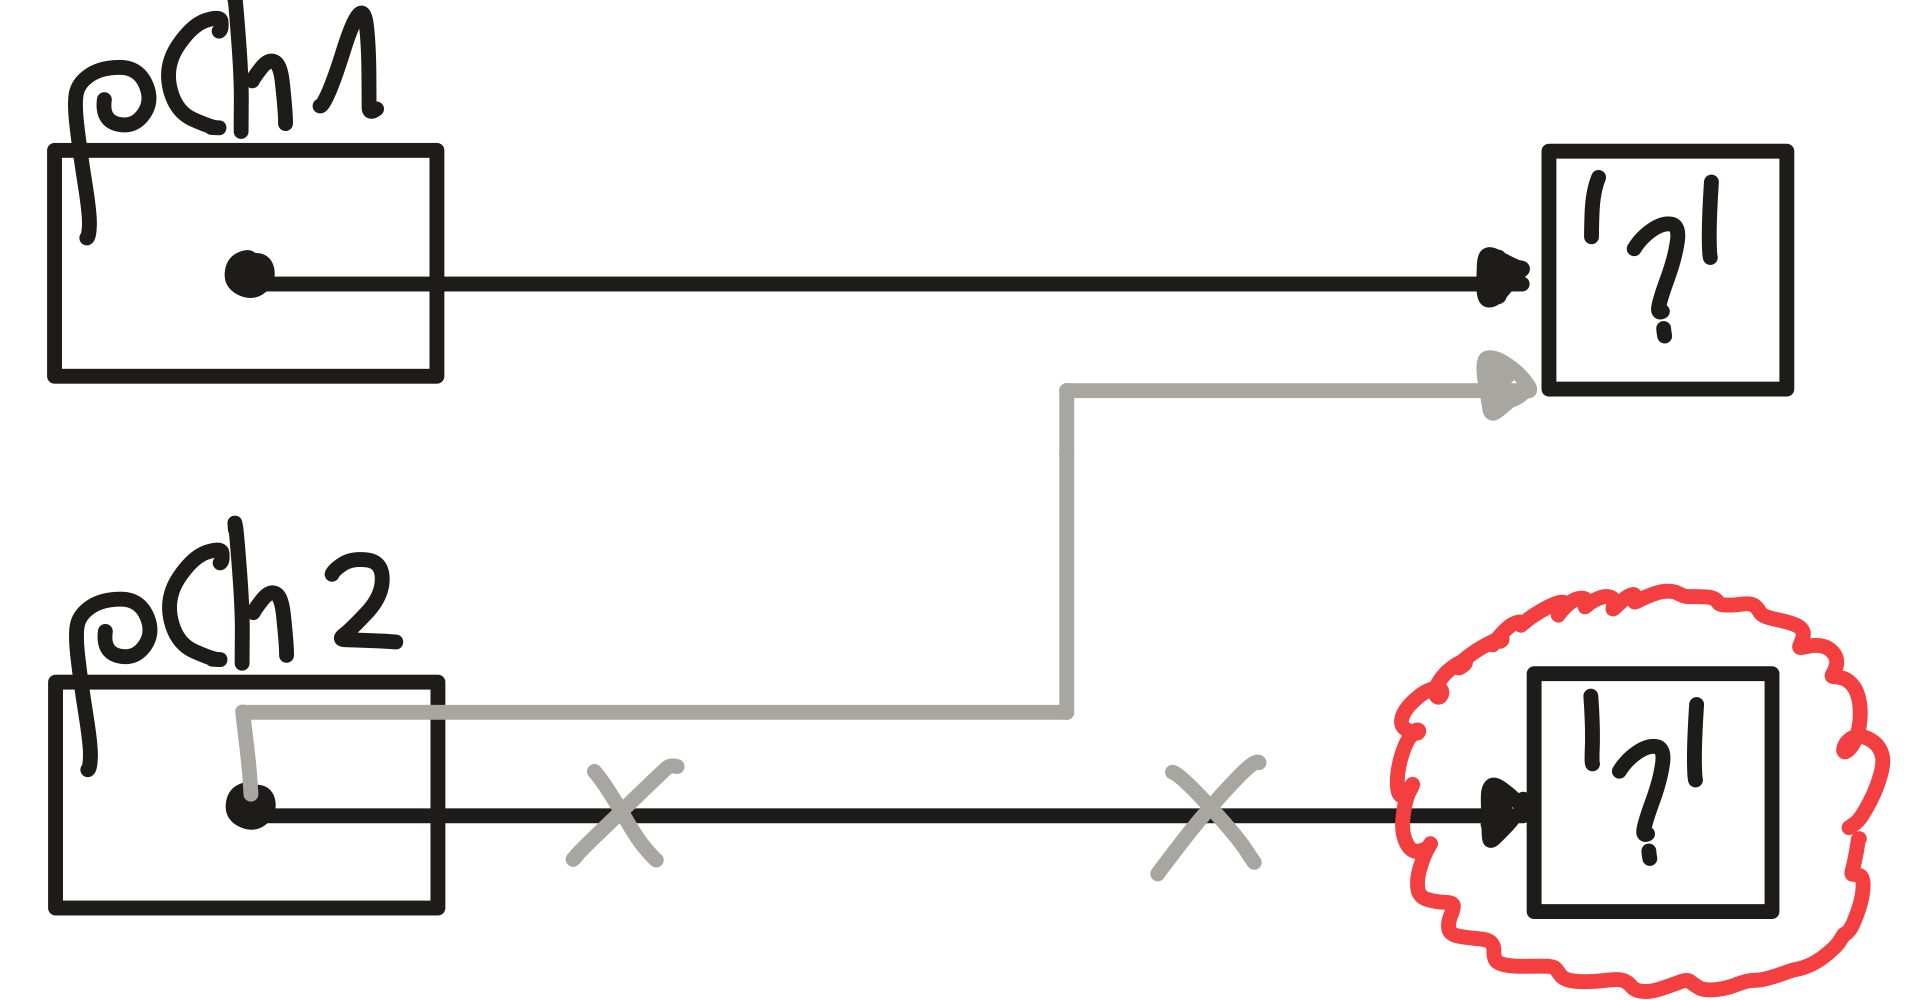
\includegraphics[width=\linewidth]{images/memory_leak.png}
\end{minipage}

\subsection{Speichermanagement funktionen}

Es gibt einige Funktionen für Speichermanagement. In C und C++ sind diese leicht verschieden. 
Generell geben diese einen Pointer zurück, welcher auf freien Speicher zeigt. 
\textbf{Diese müssen immer auf einen Nullpointer geprüft werden, da keine Garantie vorhanden ist, ob überhaupt Speicher vorhanden ist!}
Generell sollte mit solchen Pointer immer misstrauisch gearbeitet werden und nach Abschluss immer wieder freigegeben werden. 
\subsubsection{C: \texttt{malloc()},  \texttt{calloc()}, \texttt{free()}}

\textbf{malloc()} gibt einen Voidpointer(pointercasting nicht vergessen) zurück welche auf eine angeforderte Grösse an Bytes Speicher zeigt. 
Der Speicher ist \textbf{nicht} initialisiert
\textbf{calloc()} macht dasselbe, initialisiert aber den Speicher auf 0.\\
\textbf{free()} gibt den Speicherbereich wieder frei. 
\lstinputlisting{code/04_Memorymanagement/mem_mngmt_c.c}

Falls kein Speicher allokiert werden kann, wird ein NULL-pointer zurückgegeben. 
\subsubsection{C++: \texttt{new}, \texttt{delete}, \texttt{new[]}, \texttt{delete[]} (Operatoren)}

Der \textbf{new}-Operator erstellt ein Pointer welcher auf die mitgegebene Grösse zeigt. 
\textbf{new[ ]} macht dasselbe, ausser das dieser ein Array zurückgibt.

\textbf{delete} / \textbf{delete[ ]} gibt den Speicher wieder frei. 
Dieser kann auch auf den Nullpointer ausgeführt werden. 
Dieser ist \texttt{Delete} egal. 
\lstinputlisting{code/04_Memorymanagement/mem_mngmt_cpp.cpp}

\subsection{Speicheraufbau}

Der Speicheraufbau bildlich dargestellt sieht ungefähr so aus:

\begin{center}
    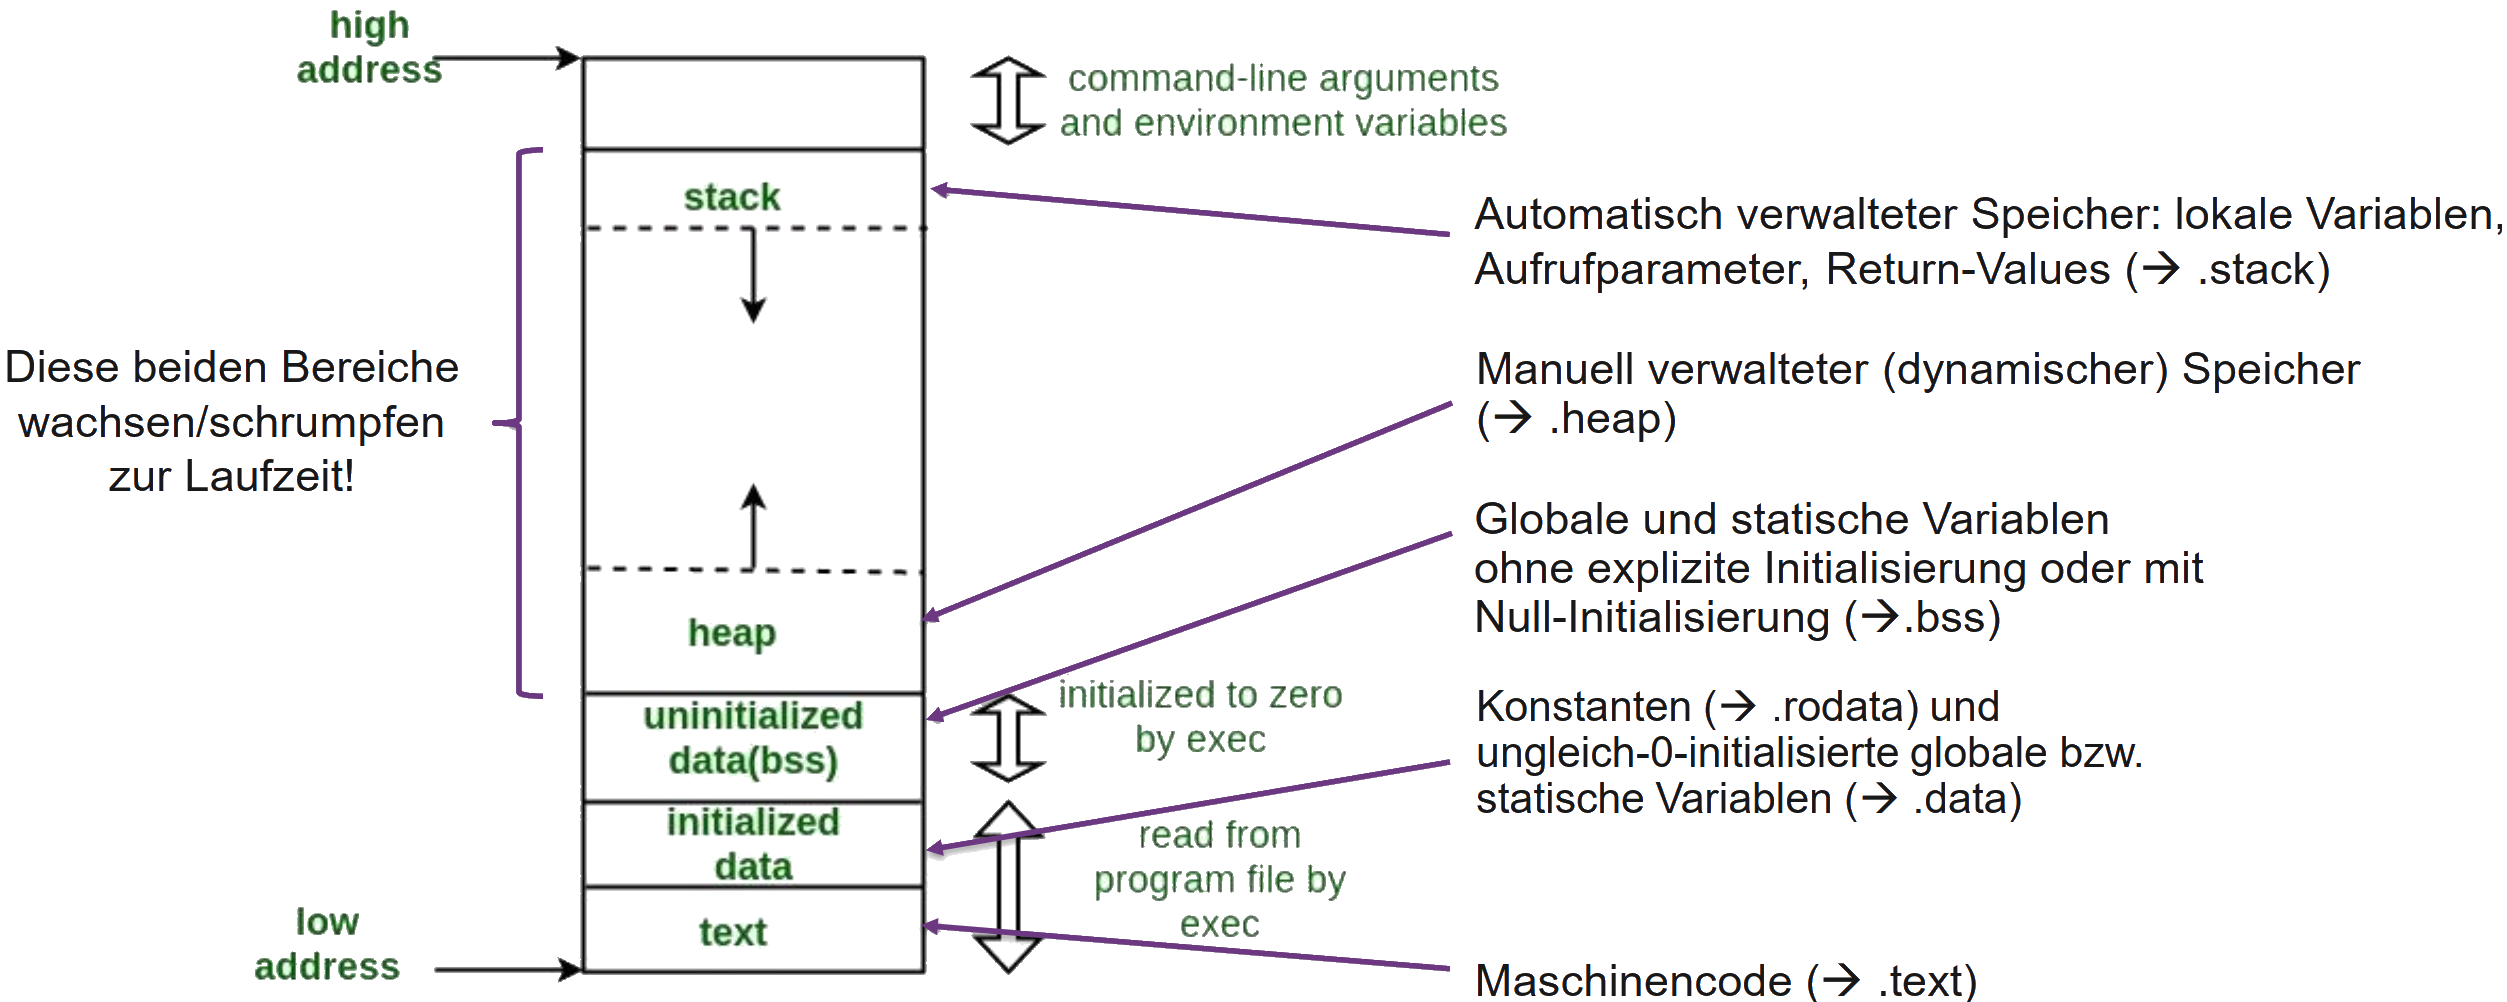
\includegraphics[width=\columnwidth]{images/memorylayout.png}  
\end{center}

Je nach Architektur kann es auch sein, dass die hohen und tiefen Adressen anders herum sind. 
\subsection{Referenzen}
Eine Referenz ist ein \textbf{Alias} (ein alternativer Name) für eine bereits bestehende Variable oder Speicherzelle.
Sie stellen eine modernere, sicherere und striktere Version von Pointern dar. 
\subsubsection{Caratteristiche Principali}
\begin{itemize}
    \item \textbf{Zwingende Initialisierung:} Muss per sofort initialisiert werden \texttt{int\& r = x;}
    \item \textbf{Unveränderlichkeit:} Darf nach Definition nicht modifiziert werden, um auf ein anderes Objekt zu zeigen.
    \item \textbf{Sicherheit:} Dürfen niemals uninitialisiert sein und besitzen niemals den Wert \texttt{nullptr}.
    \item \textbf{Effizienz:} Können in CPU-Registern liegen und belegen nicht in jedem Fall physischen Speicher. 
    Der \texttt{sizeof()}-Operator gibt die Grösse des Typs zurück, auf welchen die Referenz zeigt.
    \item \textbf{Syntax:} Werden wie normale Variablen benutzt, ohne eine Notwendigkeit zur Dereferenzierung.
    \item \textbf{Limitierung bei Arrays:} Referenzen können nicht genutzt werden, um Arrays via Arithmetik (Inkrement/Dekrement) zu durchlaufen. 
    Für genau diesen Zweck bleiben die \textbf{Pointer} unverzichtbar.
\end{itemize}

\subsubsection{Confronto: Value vs Reference}
\begin{center}
\begin{tabular}{@{}lll@{}}
\toprule
\textbf{Caratteristica} & \textbf{Call by Value} & \textbf{Call by Reference} \\ \midrule
Datenkopie          & Ja (sehr teuer bei grossen Objekten) & Nein (übergibt Alias) \\
Ändert Original      & No                             & Ja \\
Sintassi                & \texttt{void f(int a)}         & \texttt{void f(int\& a)} \\ \bottomrule
\end{tabular}
\end{center}

\subsubsection{Best Practices}
Die Nutzung von Referenzen senkt die Fehlerrisiken im Vergleich zu Pointern drastisch.
Dennoch bleiben Pointer in ganz bestimmten Fällen unumgänglich:
\begin{itemize}
    \item \textbf{Array-Verwaltung:} Ein Array "zerfällt" in Pointer auf das erste Element (\textit{pointer decay}), was Pointer zum Standard-Tool für das Durchlaufen o. Bearbeiten am Stück liegender Speicherblöcke macht.
    \item \textbf{Low-Level Programmierung:} Nötig für die direkte Hardware-Interaktion oder für die manuelle dynamische Allokation (\texttt{new}/\texttt{delete}).
\end{itemize}

\lstinputlisting{code/04_Memorymanagement/referenz.cpp}

\subsection{Speicherplatzbedarf von Objekten}

Eine Unterklasse braucht immer mindestens so viel speicher wie eine Oberklasse. 
\subsubsection{Zuweisungen}

Zuweisungen von Oberklasse zu Unterklasse sind in der regel möglich da alle geerbten Attribute ja vorhanden sind. 
Umgekehrt geht das allerdings nicht, da der Speicher dafür nicht initialisiert ist. 
\subsubsection{Slicing Problem}

\begin{itemize}
    \item \textbf{Definition:} Tritt auf, falls ein Subklassen-Objekt \textbf{als Value} einer Funktion übergeben wird, welche aber explizit eine Superklasse erwartet.
    \begin{itemize}
        \item Dabei wird jener \textit{Copy-Constructor} der Superklasse aufgerufen.
        \item Nur der "Basis"-Teil vom Objekt wird kopiert; die Erweiterungen jener Subklasse gehen verloren (Slicing).
    \end{itemize}
    \item \textbf{Conseguenza:} Innerhalb der Funktion agiert das Objekt nun exklusiv als Basisklassen-Instanz und verliert jegliches polymorphes Verhalten absolut.
    \item \textbf{Soluzione:} Nutze für die Übergabe immer \textbf{eine Referenz} (\texttt{const T\&}) oder mache es via Pointer.
    Das erhält die Integrität vom Original-Objekt und erlaubt das korrekte Funktionieren der \texttt{virtual}-Methoden.
\end{itemize}

\subsection{Type Casting}\vspace{-1em}

\begin{center}
    \rotatebox{90}{%            
    \resizebox{1.5 \columnwidth}{!}{%
    \begin{tabular}{|c|l|l|l|}
        \hline
        {\color{blue} Cast:} &
          \multicolumn{1}{c|}{{\color{blue} Anwendungsbereiche}} &
          \multicolumn{1}{c|}{{\color{blue} Wissenswertes}} &
          \multicolumn{1}{c|}{{\color{blue} Beispiele}} \\ \hline
        {\color{blue} \begin{tabular}[c]{@{}c@{}}implizit: \\ kein Cast\end{tabular}} &
      
           \begin{tabular}[c]{@{}l@{}}• Numerische Typen u. bool\\ (ggf. mit Warnung, falls Wertebereich\\ möglicherweise nicht ausreicht)\\ • Objektinstanzen einer Unterklasse in\\ einer Variablen vom Typ der\\ Oberklasse speichern (Upcast).\\ • Pointertypen, deren Umkonvertierung\\ «ungefährlich» ist – die genauen\\ Regeln sind ziemlich kompliziert.\end{tabular} &
           &
          \begin{tabular}[c]{@{}l@{}}1. {\color{codeGreen}signed char} a = 1;\\ {\color{codeGreen}int} b = a;\\ \\ 2. {\color{codeGreen}int} a = 1;\\ {\color{codeGreen}char} b = a;
 {\color{blue}// ggf. mit Warnung}\\ \\ 3. Bird b;\\ Animal a = b;
 {\color{blue}// Upcast: a ist ein Animal}\end{tabular} \\ \hline
        {\color{blue} static} &
          \begin{tabular}[c]{@{}l@{}}• Alles, was implizit möglich ist,\\ unterdrückt dabei etwaige Warnungen.\\ • Pointer- und Referenz-Typen auf\\ Instanzen von Ober- und\\ Unterklassen in beide Richtungen\\ umwandeln: Upcast und\\ Downcast (\textbf{ohne Typprüfung} zur\\ Laufzeit, Auswertung\\ ausschliesslich zur \textbf{Compilezeit})\end{tabular} &
          \begin{tabular}[c]{@{}l@{}}Um einen grösseren Integer in einen kleineren zu konvertieren, "schneidet" der Compiler überschüssige Bits einfach ab und behält nur die am wenigsten signifikanten (LSB).\end{tabular} &
          \begin{tabular}[c]{@{}l@{}}1. {\color{codeGreen}int} a = 1;\\ {\color{codeGreen}char} b = {\color{codeGreen}static\_cast}\textless{}{\color{codeGreen}char}\textgreater{}(a);\\ 2. Bird* b = {\color{codeGreen}new} Bird;\\ Animal* a = b;
 {\color{blue}// geht implizit!}\\ Bird* c = {\color{codeGreen}static\_cast}\textless{}Bird*\textgreater{}(a);\\ {\color{blue}/* Braucht einen down-Cast} , \\ {\color{codeGreen}weil nicht jedes Animal ein Bird ist!*/}\end{tabular} \\ \hline
        {\color{blue} dynamic} &
          \begin{tabular}[c]{@{}l@{}}• Pointer- und ReferenzTypen auf \\ Instanzen von\\ \textbf{polymorphen} Ober- und\\ Unterklassen in beide\\ Richtungen umwandeln:\\ Upcast und Downcast (\textbf{mit}\\ Typprüfung per RTTI zur\\ Laufzeit)\end{tabular} &
          \begin{tabular}[c]{@{}l@{}}Unterstützt ausserdem einen\\ Upcast für Pointer- und\\ Referenztypen auf nichtpolymorphe Klassen\\ (normalerweise machen wir dies aber \\ implizit oder verwenden einen static\_cast!)\\ Falls der 
 dynamic\_cast \textbf{fehlschlägt}, liefert \\ er bei Pointer-Typen den Wert\\ \textbf{nullptr}, bei Referenzen wird\\ eine \textbf{std::bad\_cast-Exception} geworfen\end{tabular} &
          \begin{tabular}[c]{@{}l@{}}Animal* a = {\color{codeGreen}new} Ant;\\ Bird* b = {\color{codeGreen}dynamic\_cast}\textless{}Bird*\textgreater{}(a);\\ {\color{blue}/* Der Dynamic Cast wird}\\ {\color{blue}immer zur Laufzeit ausgewertet. dh:}\\ {\color{blue}b ==nullptr */}\end{tabular} \\ \hline
        {\color{blue} const} &
          \begin{tabular}[c]{@{}l@{}}verändert die \texttt{constness} und/oder\\ \texttt{volatile-ness} des\\ Ziels eines Pointer oder Referenz Typs.\end{tabular} &
           &
          \begin{tabular}[c]{@{}l@{}}{\color{codeGreen}const int} val = 10;
 \\ {\color{codeGreen}const int} *ptr = \&val; \\ {\color{codeGreen}int} *ptr1 = {\color{codeGreen}const\_cast} \textless{}{\color{codeGreen}int} *\textgreater{}(ptr);\end{tabular} \\ \hline
        {\color{blue} reinterpret} &
          \begin{tabular}[c]{@{}l@{}}• Konvertiert zwischen beliebigen Pointer-Typen \\ sowie zwischen beliebigen Pointer und int-Typen \\\textbf{ohne Typprüfung}.\\ • Kann auch mit Referenz-Typen\\ umgehen.\end{tabular} &
          \begin{tabular}[c]{@{}l@{}}Achtung: erzeugt\\ plattformspezifisches Verhalten\end{tabular} &
          \begin{tabular}[c]{@{}l@{}}Animal* a = {\color{codeGreen}new} Ant;\\ \\ {\color{codeGreen}uint8\_t}* b =\\ {\color{codeGreen}reinterpret\_cast}\textless{}{\color{codeGreen}uint8\_t}*\textgreater{}(a);\end{tabular} \\ \hline
        \end{tabular}%
   
    }
    }          
\end{center}

Die C Syntax für Casting sollte nicht mehr verwendet werden da meistens nicht optimales verhalten. 
\subsection{Templates}

\begin{itemize}
\item \textbf{Typ-Unabhängigkeit:} Sie erlauben generischen Code mittels \textbf{Placeholdern} (Platzhaltern) anstelle der Nutzung von spezifischen Typen.
\item \textbf{Typen-Sicherheit (Type Safety):} Im Ggs. zu C (\lstinline|void*|) garantieren Templates eine Typenprüfung durch \textit{Early Binding} bei der Kompilation.
\item \textbf{Instanziierungs-Parameter:} Ausser Typen können auch \textbf{Konstanten} direkt als die expliziten Template-Parameter übergeben werden.
\item \textbf{Vielseitigkeit:} Dürfen auf \textbf{Klassen} wie auch \textbf{Fkt.} angewendet werden.
\item \textbf{Auswertung zur Kompilierzeit:} Der Compiler generiert den eigentlichen Code direkt während der \textbf{Compile-Time}-Phase.
\item \textbf{Struktur und File:} Erfordern Deklaration, Definition und Parameter; meist \crd{vollständig in den \textbf{Header-Files} (.h / .hpp) definiert.}
\item \textbf{Code-Erzeugung:} Der Compiler baut eine separate Kopie der Funktion oder Klasse für absolut jeden \textbf{unterschiedlichen Typ}, der genutzt wird.
\item \textbf{Zero Dead Code:} Wird ein Template nie im Code genutzt, generiert es exakt keine einzige Anweisung im allerletzten finalen Binary.
\item \textbf{Memory-Footprint und Code Bloat:} Eine Instanziierung für sehr viele Typen oder die übermässige Nutzung vom Keyword \lstinline|inline| für lange Defs. verursacht ev. \textit{Code Bloat}.
\end{itemize}

\subsubsection{Implementation}

Die Typendefinitionen sind dann durch das T zu ersetzen. 
\lstinputlisting{code/04_Memorymanagement/templatesswap.cpp}\vspace{-1.5em}

\begin{center}
  \cor{As the dimension of the paramters is unknow ALWAYS use references}
\end{center}

\subsubsection{Syntax}

\lstinputlisting{code/04_Memorymanagement/templatesyntax.cpp}\vspace{-0.5em}

\subsubsection{Instanziierung}

Instanziierung ist der Prozess, mit dem der Compiler hier dann den konkreten Maschinencode generiert\smallbreak

\begin{itemize}
    \item \textbf{Implizit:} Der Compiler leitet den Typ aus übergebenen Parametern ab. \textbf{Wichtig:} Der Return-Typ wird nie für die Ableitung berücksichtigt.
    \item \textbf{Explizit:} Der Typ wird manuell innerhalb der spitzen Klammern definiert.
\end{itemize}\smallbreak

\textbf{Klassentemplates} (\verb|<>| obbligatori):\\
Typ muss spezifiziert sein, damit der Compiler den effektiven Speicherbedarf ermitteln kann.\\
\lstinline[language=C++]|Stack<int, 10> s1; // Instanziiert einen Stack von 10 Integern|

\textbf{Funktionstemplates} (\verb|<>| opzionali se deducibili):\\
Ist der Typ via Parameter glasklar, können diese spitzen Klammern weggelassen werden.\\
\lstinline[language=C++]|int i = minimum(iF, size); // Implizite Typ-Deduktion für int|
\lstinline[language=C++]|int i = minimum<int>(iF, size); // Explizite Qualifikation|
\subsubsection{Overloading}

Die Funktions-Templates können auch mit anderen Templates oder "normalen" Funktionen überladen werden. 
Bei gleichnamigen Aufrufen wertet der Compiler kompatible Fkt. aus, instanziiert jene der Templates, fügt sie den verfügbaren normalen Fkt. bei und wählt jene Variante, die den besten \textit{Match} für Parameter-Typen bietet. 
\subsubsection{Kompilierung und Code-Organisation}
\begin{itemize}
    \item \textbf{Header-Only:} Compiler muss Def. bei jeder Übersetzung "sehen". Hauptnachteil ist eine \textbf{erhebliche Zunahme jener finalen Kompilierungszeiten}.
    \item \textbf{Explicit Instantiation (.cpp):} Um die Kompilierzeiten zu verringern, kann man Definitionen in ein \verb|.cpp|-File auslagern und Instanziierung forcieren (es. \lstinline|template class Stack<int>;|).
\end{itemize}

\section{Exceptions (Ausnahmen)}
\begin{itemize}
    \item \textbf{Error (Fehler):} Ein Implementierungsfehler. Er sollte zwingend während dem Testing/Verify behoben werden.
    \item \textbf{Exception (Ausnahme):} Eine abnormale Bedingung, welche in Runtime auftreten kann (Bsp. File fehlt, Network-Timeout).
\end{itemize}


\subsection{Meccanismo: Throw e Catch}
Eine Exception ist ein Objekt, per \texttt{throw} Keyword geworfen und per \texttt{catch} gefangen.
\begin{itemize}
    \item \textbf{Throw by value:} Diese Exceptions sollten stets zwingend per Wert geworfen werden.
    \item \textbf{Catch by const reference:} Um unnötige Kopien und das Objekt-\textit{Slicing}-Problem zu vermeiden, solltest du sie immer als konstante Referenz fangen.
    \item \textbf{Stack Unwinding:} Wurde Exception geworfen, zerstört das Programm alle Objekte (ruft Destruktoren auf) und springt direkt \textbf{zum ersten kompatiblen Handler}.
\end{itemize}

\lstinputlisting[language=C++]{code/04_Memorymanagement/exceptionGenerellSyntax.cpp}\vspace{-1em}

\subsection{Propagazione (Exception Propagation)}
Wird eine Exception lokal nicht gehandelt, reicht man sie "nach oben" weiter (z.B. auf die Applikations-Ebene), wo ein sinnvoller Entscheid fällt (Grundsatz: Handle nur das, worüber du entscheiden kannst). 
\begin{itemize}
    \item Innerhalb von einem \texttt{catch}-Block wirft die \texttt{throw;}-Instruktion (ganz ohne Argumente) die genaue, aktuelle Exception erneut an die aufrufende Funktion.
\end{itemize}

\subsection{Gerarchia e Ordine dei Catch}
In C++ werden Exceptions hierarchisch unter der Basisklasse \texttt{std::exception} (ist in \texttt{<exception>} definiert) angeordnet. 
\begin{itemize}
    \item \textbf{logic\_error: \crd{NICHT BENUTZEN}} Fehler, die in der Entwicklung vermeidbar sind
    \item \textbf{runtime\_error:} Unvorhersehbare Fehler in Folge von externen Ereignissen\\
    (es. \texttt{overflow\_error}, \texttt{system\_error}, \crd{includere \texttt{stdexcept}}).
\end{itemize}

\medbreak

\textbf{\color{orange}Cruciale Regel:} Handler müssen zwingend von sehr spezifisch zu sehr generisch im Code geordnet sein. \texttt{std::exception} oder der Catch-All \texttt{...} ist am Schluss.

\begin{lstlisting}{language=C++}
catch(...) {/* Catch everything */}
\end{lstlisting}

\resizebox{\columnwidth}{!}{
\input{tikz/exception_table.tex}
}

\example{}
\lstinputlisting[language=C++]{code/04_Memorymanagement/catchcatcher.cpp}\vspace{-1em}

\subsection{Eccezioni non gestite}
Wird absolut gar kein gültiger Handler im \textit{Call Stack} gefunden:


\begin{enumerate}
    \item Wird nun die Funktion namens \texttt{std::terminate} gerufen.
    \item \texttt{std::terminate} ruft einen \texttt{terminate\_ handler} (Default ist \texttt{std::abort}).
    \item Das Programm endet jetzt ziemlich brüsk (kein Ausführen der Destruktoren)
\end{enumerate}\smallbreak

Es ist möglich, dieses Verhalten spezifisch über \texttt{std::set\_terminate()} anzupassen. 
\subsection{noexcept}
\begin{itemize}
    \item \textbf{noexcept:} Eingeführt in C++11, zeigt es, dass Fkt garantiert keine Exceptions wirft. Dies ist sehr nützlich für die Optimierung des Compilers.
    \item \textbf{Operatore noexcept(expr):} Gibt exakt \texttt{true} zurück, wenn die Expression als \texttt{noexcept} deklariert ist.
\end{itemize}

\lstinputlisting[language=C++]{code/04_Memorymanagement/noexcept.cpp}\vspace{-1em}

\subsection{C++ e Low-Level Exceptions}
Anders als in Java oder C\# übernimmt die Sprache C++ \textbf{kein} auto \textit{Mapping} jener Low-Level Exceptions (wie z.B. bei der Division durch Null) in normale Sprach-Exceptions. 
\smallskip

Handling con \texttt{catch(...) \{ \}} 

\section{STD Library}
\subsection{array}
\begin{itemize}
\item \textbf{Definition:} \texttt{std::array<T, size>} ist ein Container von absolut fester Grösse implementiert als Template-Klasse.
\item \textbf{Dimension:} \texttt{std::array} weiss seine ganz exakte Dimension aus der Memberfunktion \texttt{.size()}.
\item \textbf{Zugriff auf Daten:} Klassische eckige Klammer Notation in \texttt{[]}.
\item \textbf{Sicherheit:} \texttt{.at()} greift dank Limit-Check sicher zu, Exeption \lstinline|std::out_of_range| tritt bei einem ungültigen Zugriff auf.
\item In den Parametern von Fkt übergebbar als eine \textbf{\color{red}Referenz, ist stets zu tun} (da es ja Klassen sind)
\end{itemize}

\example{}
\lstinputlisting[language=C++]{code/04_Memorymanagement/standart_array.cpp}\vspace{-1em}

\subsubsection{Matrix}
\begin{itemize}
\item \textbf{Struktur:} Externe Dimension: Zeilen, intern: die Spalten.
\item \cor{Erfordert zwei Doppel-Paare an geschweiften Klammern zum Initialisieren (weil dieses \texttt{std:array} eine Klasse ist)}
\item \textbf{Zugriff:} Doppelte Index Notation: \texttt{matrix[riga][colonna]}.
\end{itemize}

\example{}
\lstinputlisting[language=C++]{code/04_Memorymanagement/standart_matrix.cpp}

\subsection{vector}
std:vector ist ein Klassentemplate welches die Kapazität selbständig bei Bedarf erweitert.
\lstinputlisting{code/04_Memorymanagement/vector.cpp}